\chapter{Delivering conventional tides to compliment modern applications}
%-----------------------
\begin{quote}
{\small
Using the Australian setting, this chapter asserts that conventional tide prediction services can better compliment modern applications by adopting appropriate data categories for machine-to-machine delivery.  It is written from the premise that the notion of such a service would represent a significant conceptual shift for conventional practice. Furthermore, incremental changes in this direction are feasible and would facilitate future improvements. In putting this case, emphasis is placed on clarifying easily confused tidal concepts and especially on the distinguishing official predictions from physical estimates. Three basic problems are outlined: (1)difference of representational aims from tidal models (2) the risk of double counting and (3) discontinuous evolution of parameters.  Whilst nuanced but known to specialists, each can become significant in certain scenarios for an operational service.  A national automated tidal data service would helpfully distinguish between the well established roles for ``official'' tides, forecasting and various auxiliary applications. Demonstrative evaluations are carried out using an archive of analysis parameters from the Australian National Tidal Unit, ocean circulation forecasts and the TPXO global tide solution. A realistic set of data categories are proposed that would facilitate automated delivery but avoid the pitfalls described.
}
\end{quote}

\label{chp:tideFlavours}
%----------------------------------------------------------
% content variables
%----------------------------------------------------------
% define variables for antt station ids used in figure names
\newcommand{\Ba}{63540}
\newcommand{\Ca}{46290}
\newcommand{\Da}{62430}
\newcommand{\Ea}{62290}
\newcommand{\Fa}{61561}
\newcommand{\Ga}{57720}

\newcommand{\Bb}{529020}
\newcommand{\Cb}{200970}
\newcommand{\Db}{005096}
\newcommand{\Eb}{008314}
\newcommand{\Fb}{523757}
\newcommand{\Gb}{200854}

\newcommand{\Bname}{Mornington Island}
\newcommand{\Cname}{Christmas Island}
\newcommand{\Dname}{Point Murat}
\newcommand{\Ename}{Geraldton}
\newcommand{\Fname}{Cape Jervis}
\newcommand{\Gname}{Lord Howe Island}

%------------------------------------------------
% main
%------------------------------------------------
\section{Chapter introduction}
\label{Sec:intro}
%--------------------------
This discussion makes the case that conventional tide prediction services will better compliment modern forecasting by adopting appropriate data categories for machine-to-machine delivery.  It is written from the premise that the notion of such a service would represent a significant conceptual shift from conventional practice.  The introduction characterises the place of conventional tidal prediction within an operational agency with diverse uses beyond navigation. Three problems for a prospective data service are described; (1) section \ref{Sec:OfficialGlobal} highlights the different representational aims of standard tides and physical tide models with respect to the underlying physics ;(2) section \ref{Sec:DoubleCount} addresses the implications of including meteorologically dominated tides and double counting signals in hybrid applications; and (3) section \ref{Sec:Evolution} describes the intentional discontinuities in annual tidal parameter updates across the historical archive of Australian operational data.   Finally Section \ref{Sec:proposed} proposes a minimal set of data ``flavours'' that could help ensure an automated machine-to-machine tide service best compliments the modern requirements. 


\subsection{Modern data micro-services and earth system modelling}
National forecasting agencies are increasingly providing machine-readable online data to support the diverse downstream economy of value-adding applications.
This `micro-service' architecture \citep{BCG2020} is increasingly relevant to government services across the board \footnote{\url{api.gov.au}} and more specifically for tides to the International Hydrographic Organisations navigation-focused exchange specifications \footnote{\url{http://s100.iho.int}}.

 
At the same time, earth system model forecasting continues to increase in sophistication along the dimensions of representational 'concreteness' \citep{Petersen:2012kp}, forecast duration, assimilation of observations and combination into seamless services \citep{BOM2020}.
Within this context, coastal sea level is the subject of a diverse range of productive development activity often centred on high resolution numerical simulations and real-time observations \citep{10.3389/fmars.2019.00437}. 


Despite all the advances in earth system modelling, conventional tide prediction remains a unique and persistent form of forecast that is well-suited to on-demand delivery.  Tide predictions are an input to many systems, have relatively tiny data volumes and are built on a conceptual foundation that allows for cheap synthesis of timeseries at arbitrary times.    There are several examples of on-demand machine-readable tidal data service \footnote{such as  \url{https://tidesandcurrents.noaa.gov/tide_predictions.html}} but nothing yet from an Australian agency and none that are known to distinguish variants for different applications.


Automated delivery of conventional tidal data raises the attractive potential to synthesise tidal timeseries at any arbitrary times as required by an application; whether that time be in the past or the future.   But there is a risk that a naive implementation of such a service may unfortunately re-enforce conceptions that tidal sea levels are an uncomplicated data type without what could be called a range of ``flavours''.
Whilst the precise details of tidal data may be irrelevant for many applications, the following discussion highlights why tidal data would be better treated like other analysis and forecast services by clearly distinguishing some variants or data ``flavours''. 
Appropriate distinction of tidal data types would clarify the compatibility of the content whilst allowing developers and users to remain relatively isolated from backend details and processing improvements on the part of the supplying agency.

%--------------------------
\subsection{Why conventional tide predictions are still relevant}
Given the ongoing advances in both observation and simulation, it would be reasonable to assume that conventional tide prediction services have been rendered redundant; but that is not the case. 
Conventional tidal sea level products are well embedded into coastal economies.   The utility of accurate predictions on a sub-hourly timescale provided over multi-year forecast horizons is unique and this reflects the typical dominance of tidal signals in coastal sea level.
Godin colourfully remarked that when inspecting spectra of observed sea level variability from tide gauges ``the [tidal] constituent lines emerge from the noise background as trees from the grass'' \citep{godin:1972}.
The ability to fit and exploit time-invariant admittance relationships between the patterns of astronomical motions and observed sea level records is an early and great success of mathematical geophysics \citep{Cartwright:2000tt}.  Harmonic tidal analysis derives unique ``\textit{forecasting power.. from the infinite extent of its basis functions} ''\citep{Flinchem:2000kp}.
Conventional products such as tide tables are however so well embedded and useful as to be somewhat taken for granted or used in isolation from other information. 

\subsection{National agency practice and diverse uses}
In Australia, harmonic tidal analysis and prediction have been routine business for government agencies for several decades.  For navigation purposes the Australian Hydrographic Service promulgates an annual official set of port predictions in the form of the Australian National Tide Tables (ANTT) and its software version AusTides \citep{austides}.  AusTides is not an automated data delivery service, but rather stand alone electronic version of the tide tables.  
The majority of the analysis behind the tide tables is carried out by the Bureau of Meteorology National Tidal Unit.  
The analyses are founded on a harmonic least-squares method implemented within a proprietary suite of software that traces a lineage to what was then known as the Proudman Oceanographic Laboratory in Liverpool \citep{MHL2156,Cartwright:2000tt}.    
The Bureau and various other state agencies publish annual tide predictions at locations additional to the ANTT. 
This well established practice of routine harmonic tidal analysis and prediction will be called ``conventional''.


The downstream application of these tidal sea-level products is not however limited to navigation.   
In fact, the range of contemporary uses motivates the present discussion; for instance:
\begin{inparaenum}[1)]
    \item land survey and cadastral references - mean sea level and tidal planes such as ``highest astronomical tide'' 
    \item hydrographic survey, charted depths and clearances
    \item long term planning for coastal works and installations
    \item short term forecasts for coastal activities 
    \item filtering (de-tiding) of sea level observations
    \item input into data-driven decision support systems
    \item combination with physical forecasts into seamless water level forecasts 
    \item verification and tuning of hydrodynamic modelling
\end{inparaenum}

A notable aspect of national tide services is the special status of promulgating predictions that have official status \citep{AusNavAct2012}.   For some applications it could be argued this status is more important than forecast accuracy alone.
  

Conventional tidal analysis has some unique and attractive features from an operational maintenance perspective.
At face value, the practice is robust to data-stream indeterminacy,  and has established methods for exploiting heterogeneous, poor quality and historical observations to produce useful predictions.  
Operational support of an annual batch-mode production schedule is far less demanding than real-time continual forecast systems. 
Furthermore, the fact that harmonic methods compress results to a few dozen human-readable parameters that are amenable to routine quality checking and error detection is also operationally attractive. 
Conventional tidal analysis at port locations can be characterised as a slow-motion data-driven method that is somewhat physics-free; especially when compared to modern hydrodynamic simulations. 

Figure \ref{fig:tidePractice} portrays the unique way that conventional tidal practice can transform heterogeneous historical records into a consistent timeseries product at arbitrary time sampling.
The pragmatic role of experts in managing what is now commonly  called ``data wrangling'' and merging non-uniform and auxiliary sources is a notable contrast to fully automated systems.
 
\begin{figure}[!hbt] \centering
        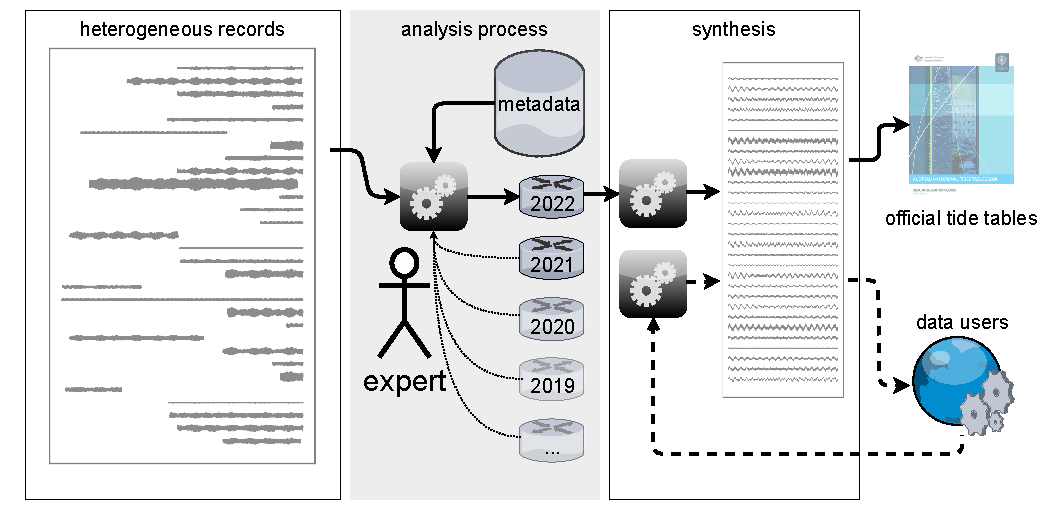
\includegraphics[width=\figwidthFull]{figures/diagrams/tideSchematic.pdf} 
        \caption{Conventional operational tide prediction update process}
        {Schematic illustrates how a conventional tidal process manages heterogeneous data sources on an annual update cycle.  Official tide requirements are not identical to those of all data users.  Dotted lines indicate the potential for on-demand synthesis.}
        \label{fig:tidePractice}
\end{figure}   


Growing access to real-time quality observations both remote and insitu has potential to tip the balance of value away from conventional tidal and even physical simulations at shorter timescales (eg \citep{10.3389/fmars.2019.00437}, \citep{10.3389/fmars.2020.00260} ), but it will be difficult to displace at the longer scales of months to years that conventional products are relied upon.
Furthermore the pragmatic matters of applying real-time quality control, managing data source inhomogeneity and the relatively sparse spatial coverage remain non-trivial problems in Australia viewed from a national perspective.


Even if the unique properties of conventional tide products seem to guarantee some ongoing relevance, the following discussion makes a case for ensuring that conventional tide products are delivered in a manner that is fit-for-purpose without inviting needless representational error. 


%--------------------------
\subsection{Precedents for data differentiation}

Most simply, the distinction between a forecast and an ``analysis'' would not be possible if an automated tidal service provided a single all-purpose synthesised signal.
This distinction is obvious to users of weather forecast data and other oceanographic products \footnote{(eg \url{https://marine.copernicus.eu/})} but arguably tidal predictions have to date maintained an exceptional product status.  Tides in general are commonly thought of as being much more akin to astronomical phenomena than oceanographic model outputs \citep{Jay:2003bj} \citep{10.1029/2018rg000636}.


The operational delivery of remote  observations of sea level has well established distinctions between what could be called data `flavours'.   Both with regard to the distinction between rapid update interim products and behind-real-time quality analysis as well as the wide range of geophysical  correction combinations that are suited to different applications (eg \citep{Scharroo:2014vv} )


Allowing for the effective operational use of standard tide products in the context of satellite observations raises the significance of basic compatibility 
issues such as vertical reference datums \citep{10.3389/fmars.2020.549467}.
Similarly, whilst remote observations of sea level anomalies (SLA) are a critical constraint on operational non-tidal forecasts \citep{10.1080/1755876x.2019.1685834}, any extension to render tide gauge data into the same format would require compatible tidal corrections - and corrections differ in intent from official port predictions.


%------------------------------------------------
\section{Problem 1: different conceptions of tidal}
\label{Sec:OfficialGlobal}
Standard tide predictions and spatial (eg gridded) tide solutions are in parallel use within ocean forecasting but do not aim to represent exactly the same phenomena.    The potential for this to be problematic is apparent in the case of global tide solutions. 
Global tide solutions are a foundational oceanographic product that in rough approximation extends the tradition of tidal analysis well away from tide gauges.   Similar to conventional tidal techniques, these solutions conceptualise the ocean as a linear-time-invariant (LTI) system forced by the tidal gravity patterns. Whilst production of the solution typically involves a hydrodynamic component\citep{Egbert:2002ug}, the result is effectively the spatial equivalent to a set of static conventional tidal parameters.   The surface height predictions from global tide solutions allow for the decomposition of remote ocean observations into tidal and nontidal components, but are also widely used for other extension applications.
In contrast to the advancing ability of physical ocean circulation forecasts to explicitly include tides (eg \citep{10.1016/j.ocemod.2019.02.008}), global LTI tide solutions share the unique ability of conventional prediction methods to efficiently provide data at the arbitrary times required by the application.


For instance, the national inter-tidal extent mapping exercise of \citet{10.3390/rs10030480}  directly applied global model predictions in part for the machine-readable and on-demand availability.
Various Australian studies of water level \citep{Haigh:2013bn}\citep{Pattiaratchi2018} and more recently currents \citep{10.5194/os-2020-107} all apply timeseries synthesised from global model solutions to provide model boundary conditions at what ever time period is required.    Such simulations add value at the time and length scales afforded by higher spatial resolution, but the longer scales require special handling that bring to attention the manner in which the aims of physical models and standard predictions differ.

\subsection{Intentional differences - especially for long period tides}
Harmonic developments of the tidal potential include a relatively weak species referred to as the long period tides.  Some of the long period constituents are known by conventional names such as \textbf{Sa}, \textbf{Ssa}, \textbf{Mm},\textbf{Msf} and \textbf{Mf}; see \citep[table 4]{agnew2015}.
Conventional tidal prediction applies essentially the same statistical fitting procedure to the long period tides as to the more familiar higher frequency tidal periods; though usually with some inclusion caveats based on the observational record. 
But regardless of record length, the treatment of long period tides highlight a difference in the aims of conventional tide prediction and modern tide models.   Namely the extent to which it is desirable to fit patterns that are primarily the result of non-astronomical phenomena.
Parker's tide manual states that ``\textit{whether the calculated values of Sa and Ssa are used or not, becomes almost a philosophical question...and may not represent the annual cycle for a particular year very well anyway}''  \citep[Section 3.7]{Parker:2007wq} 

Physical approaches to the quantifying global long period tides \citep{Egbert:1994wz} do not result in amplitudes anything like those resulting for conventional tide gauge records; especially for when relatively short records and significant nontidal power noise is involved.   Amplitudes of over 20cm are attributed to long period tides in places along the Australian coast as shown in Figure \ref{fig:SaAmp}. In contrast to the aim of physical attribution, when an annual forecast of sea level is the target it is understandable that \textit{any} pattern found to be periodic enough to project onto the tidal basis functions is included in the synthesis of the prediction. 

Even if this intentional difference is known to specialists, downstream users of an automated tidal data service are at risk of building in needless representational error if the distinction is not designed clearly into the service.
The nature of tidal analysis is such that the distinction is best not conceptualised as simply high versus low frequency, but rather physical versus periodic.   The periodic but not gravitationally forced patterns have historically been termed `radiational' tides \citep{agnew2015}.  So the situation outlined for the long period tides also exists for the generally tiny but weather-dominated daily constituent \textbf{S1} \citep{Ray:2004ts}.
 
% Amp
\begin{figure}[!hbt] \centering
    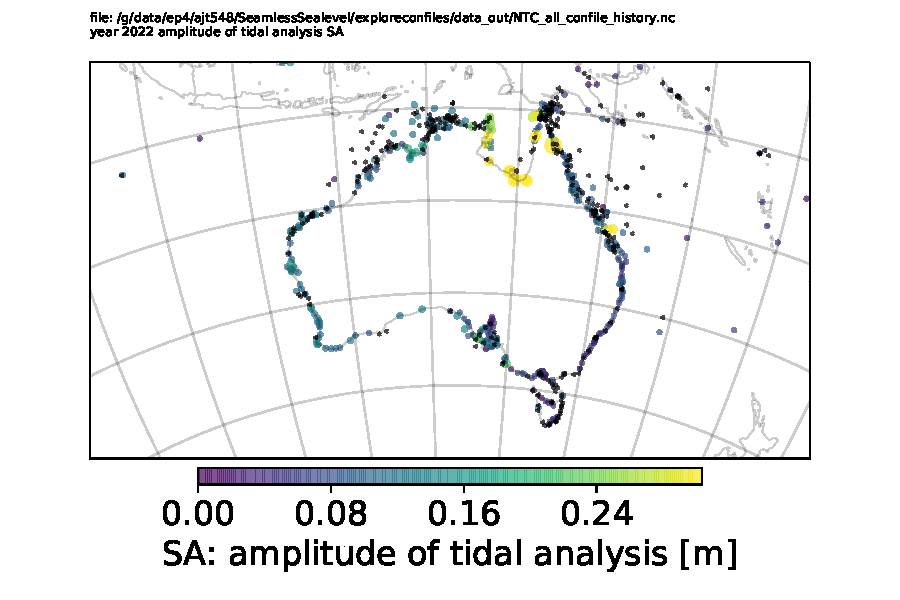
\includegraphics[trim={0 0 0 1cm},clip,width=\figwidthBig]{figures/maps/locations_SaAmp.pdf} 
    \caption{Amplitude of \textbf{Sa} at analysis locations}
    {Amplitude of \textbf{Sa} at analysis locations. Over 650 mixed-quality stations are on record.}
    \label{fig:SaAmp}
\end{figure}

% Pha
\begin{figure}[!hbt] \centering
    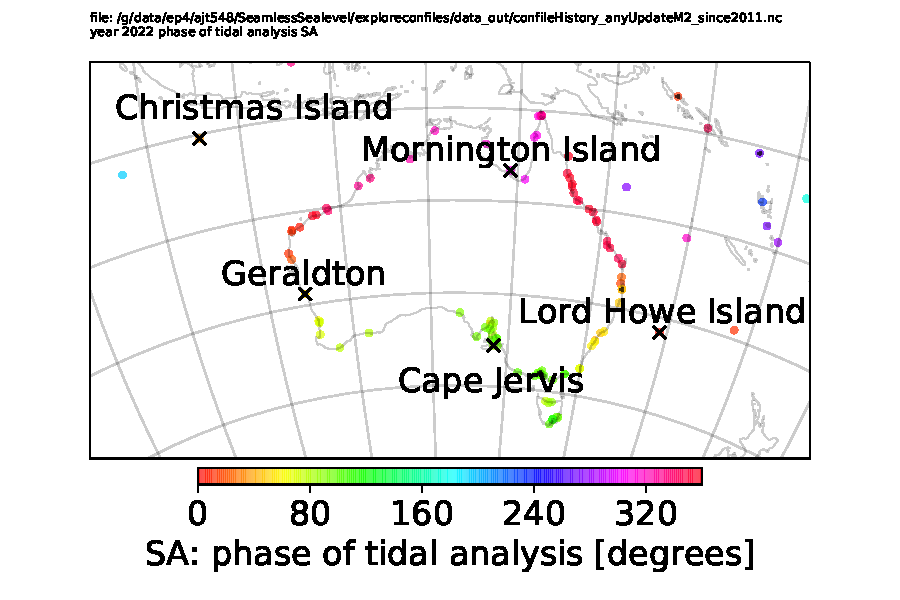
\includegraphics[trim={0 0 0 1cm},clip,width=\figwidthBig]{figures/maps/locations_SaPhaAnyM2Update.pdf} 
    \caption{Phase of \textbf{Sa} at analysis locations}
    {Compared to Figure \ref{fig:SaAmp}, only 132 stations have recently updated analyses. Location names used in text are also shown. Note that there are different conventions for allocating Doodson codes that influence interpretation of these phase values \citep[10.4]{PCTMSL-sp9}}
    \label{fig:SaPha}
\end{figure}   

In contrast to conventional tidal analysis, the widely used Oregon State University Tide Prediction Software \citep{Egbert:2002ug} [hereafter \textbf{TPXO}] totally excludes Sa, Ssa, Msf and S1; but both include Mm and Mf.  Subsequently any application that brings both type of prediction into the same context, even if indirectly, requires some caution to avoid representational inconsistency. 


\subsection{Inter-representation agreement}
Given that the signal amplitudes are generally rather small and that most tidal evaluations are carried out in frequency space, the following evaluation aims to demonstrate the practical implications when handling synthesised timeseries.

Variants of 15 minute tide predictions at all Australian sites for the full year of 2020 are used for comparison. TPXO predictions were generated using the standard interpolation to site locations and sites where excluded that fell beyond the solution grid.   The National Tide Unit in-house software (unpublished) was modified to selectively exclude particular constituents in order to generate alternative ``standard'' predictions for the study period.  All prediction time series for this comparison are relative to MSL (more on that in Section \ref{Sec:MSL}).   Both systems apply so-called nodal or satellite corrections to modulate a finite list of constituent parameters.   

It is to be expected that a global tide solution will not represent all the localised and shallow-water patterns that a conventional analysis can capture.   However the aim of this evaluation is to highlight the arguably less-expected but intentional representational difference for primarily meteorological tides.   To this end, the following timeseries comparison metric is shown on the summary map in Figure \ref{fig:improveOtps}.
\begin{equation}
    I = 1- \frac{rms(\eta_{B}-\eta_{TPXO})}{rms(\eta_{A}-\eta_{TPXO})}
    \label{eq:improvment}
\end{equation}
With water level timeseries $\eta$ variants:
\begin{inparaenum}
[A)]
    \item port tides with all constituents; 
    \item port tides with excluded constituents individually and in combination: Sa, Ssa, Mm, Msf, Mf and S1.
\end{inparaenum}
Increasingly positive values for the metric $I$ reflects improved agreement between the insitu and the global tide solution by the exclusion of constituents.  A null value reflects no change, and negative $I$ reflects decreased agreement.


The \textit{total removal} of the selected constituent terms consistently improves the compatibility of the physical and conventional predictions as is expected.   Moreover, improvement in agreement is partially contributed by each individual constituent with the only case for any ambiguity being \textbf{Mf}; visualised in Figure \ref{fig:improveOtps} panel [b]. Mf is the strongest of the long period forcing terms but still overall these results indicate that the conventional tide attribution is skewed towards the projection of nontidal noise (see Figure \ref{fig:williamsFraction} panel [e] as well). 

As an example of the practical implications of such compatibility, consider the role of conventional tidal planes such as Highest and Lowest Astronomical Tide (HAT and LAT).  Whereas these planes are derived at port locations based on standard predictions that include radiational tides, any spatial extension of the planes that involves a physical tide model risks systematic disagreements of order 10-20cm.  


\begin{figure}[!hbt] \centering
    \begin{subfigure}[b]{\figwidthHalf}
        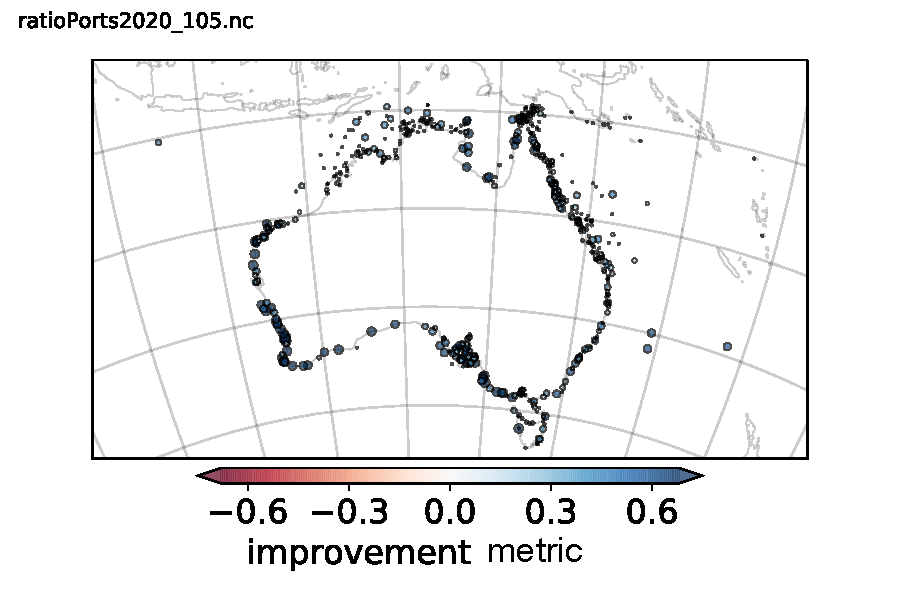
\includegraphics[trim={0 0 0 1cm},clip,width=\textwidth]{figures/maps/otpsPortCompare_Improve2020_105_diffRmse.pdf}
        \caption{Metric $I$ evaluated for variant excluding nominally weather dominated consituents.}
    \end{subfigure}
    \begin{subfigure}[b]{\figwidthHalf}
        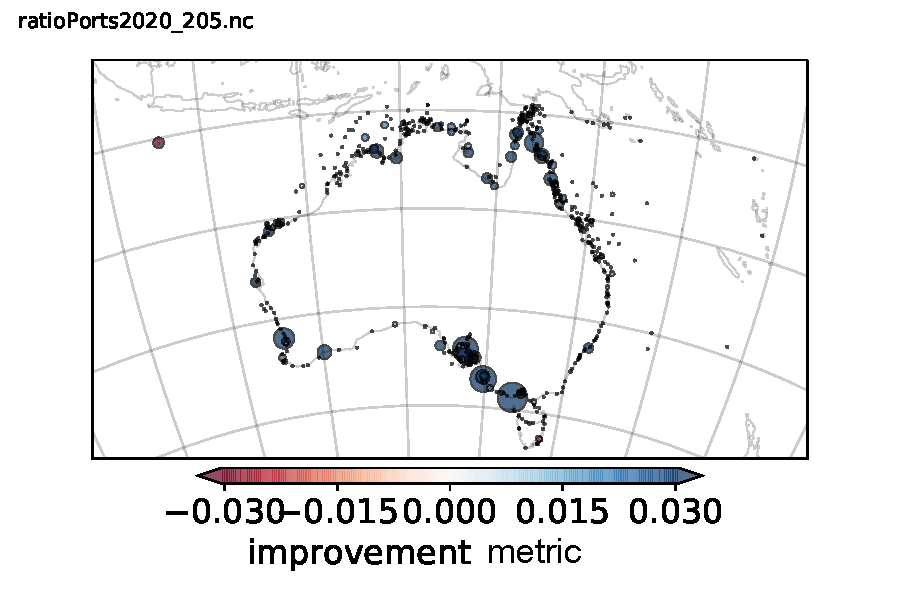
\includegraphics[trim={0 0 0 1cm},clip,width=\textwidth]{figures/maps/otpsPortCompare_Improve2020_205_diffRmse.pdf}
        \caption{Same as (a) for variant excluding \textbf{Mf} alone - note scale}
    \end{subfigure}
    \\
    \begin{subfigure}[b]{\figwidthThird}
        \includegraphics[width=\textwidth]{figures/plots/compareTides_\Fa_Full2020.pdf} 
        \caption{Timeseries scatter for 1 year of hourly port tide predictions against OTPS/TPXO}
    \end{subfigure}
    \hfill{}
    \begin{subfigure}[b]{\figwidthThird}
        \includegraphics[width=\textwidth]{figures/plots/compareTides_\Fa_2020_201.pdf} 
        \caption{Same as (c) for insitu prediction variant excluding only the annual cycle constituent \textbf{Sa}}
    \end{subfigure}
    \hfill{}
    \begin{subfigure}[b]{\figwidthThird}
        \includegraphics[width=\textwidth]{figures/plots/compareTides_\Fa_2020_105.pdf} 
        \caption{Same as (c) for case excluding all nominally weather dominated constituents}
    \end{subfigure}
    
    \caption{Representational agreement between global tide model and port tides evaluated on hourly predictions for the year 2020.}
    {Panels a-b show unitless metric $I$ evaluated for two port prediction variants;  consistency between TPXO tide model and 'official' port tides is improved by total removal of weather dominated constituents from the later.  Panels c-e illustrate underlying data for the single location of \Fname{} by presenting scatter comparison of predicted heights relative to MSL for selected port prediction varients.  See Figure \ref{fig:SaAmp} for \textbf{Sa} amplitudes.}
    \label{fig:improveOtps}
\end{figure}   


%------------------------------------------------
\section{Problem 2: double-counting in hybrids}
\label{Sec:DoubleCount}
A practical implication of facilitating downstream applications to access tidal data is the risk of ``double-counting'' signal; especially when hybridising tide data with physical models. 
\citet{os-14-1057-2018} described this risk and made evaluations based on the tidal analysis of global barotropic ocean simulations for single one year period. 
The supplementary data supplied by Williams are used to visualise the power projected by wind and pressure effects onto standard tidal constituents in Figure \ref{fig:williamsFraction}.  The spatially consistent high ratios for long periods and S1 stands in stark contrast to the small fractions attributed to the other constituents (not shown).    
For the purposes of providing a tidal data service that can facilitate hybrid applications (eg \citep{Taylor:2017coa}) whilst mitigating double-counting, these evaluations suggest that simply excluding the long periods and S1 in total would be a reasonable starting point.   This is discussed further in  section \ref{Sec:proposed}.
This simple interpretation of the Williams evaluation intentionally underplays the details of phase and wave interaction effects to focus on the gross differences in representational aim between physical models and standard tide predictions. 
The ``\textit{possibility that ... non-tidal power is leaking into the Mm and Mf estimates}'' in this short model analysis adds to the expectation that such leakage is a dominant effect for many Australian tide prediction sites, especially given that a barotropic ocean model evaluation excludes the role of steric and ocean circulation phenomena projecting onto tide predictions; discussed further in section \ref{Sec:Evolution}.

It is notable that long period signals in Australian sea level studies have always been subject to careful ``non-tidal'' treatment. For instance \citet{Haigh:2013bn} and \citet{Pattiaratchi2018} ensure that long period signals are appropriately filtered, fit or replaced to account for the representational limits of the respective models when interpreting results against observations.

\begin{figure}[!hbt] \centering
    \begin{subfigure}[b]{\figwidthHalf}
        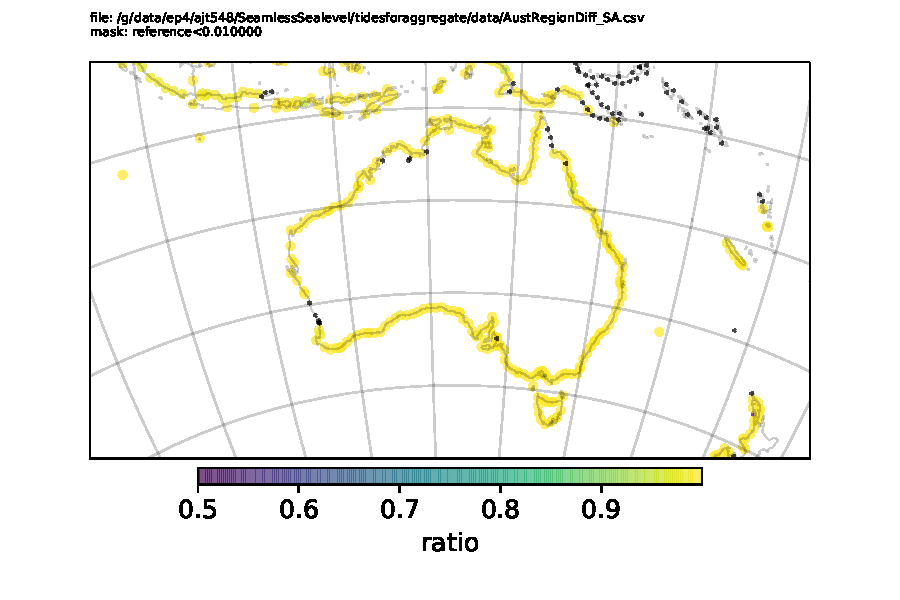
\includegraphics[width=\textwidth]{figures/maps/AustRegionDiff_SA.pdf}
        \caption{Sa}
    \end{subfigure}
    \begin{subfigure}[b]{\figwidthHalf}
        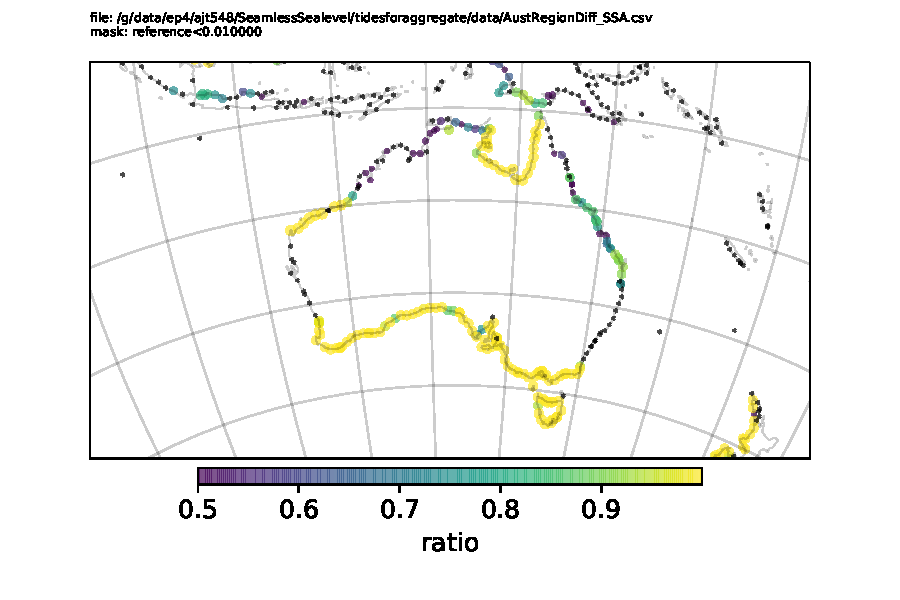
\includegraphics[width=\textwidth]{figures/maps/AustRegionDiff_SSA.pdf}
        \caption{Ssa}
    \end{subfigure}
    \begin{subfigure}[b]{\figwidthHalf}
        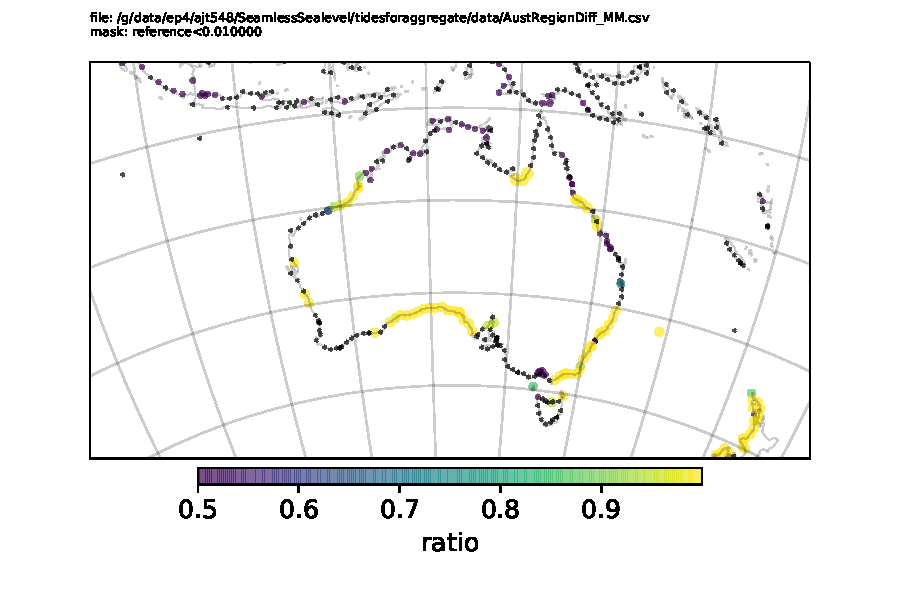
\includegraphics[width=\textwidth]{figures/maps/AustRegionDiff_MM.pdf}
        \caption{Mm}
    \end{subfigure}
    \begin{subfigure}[b]{\figwidthHalf}
        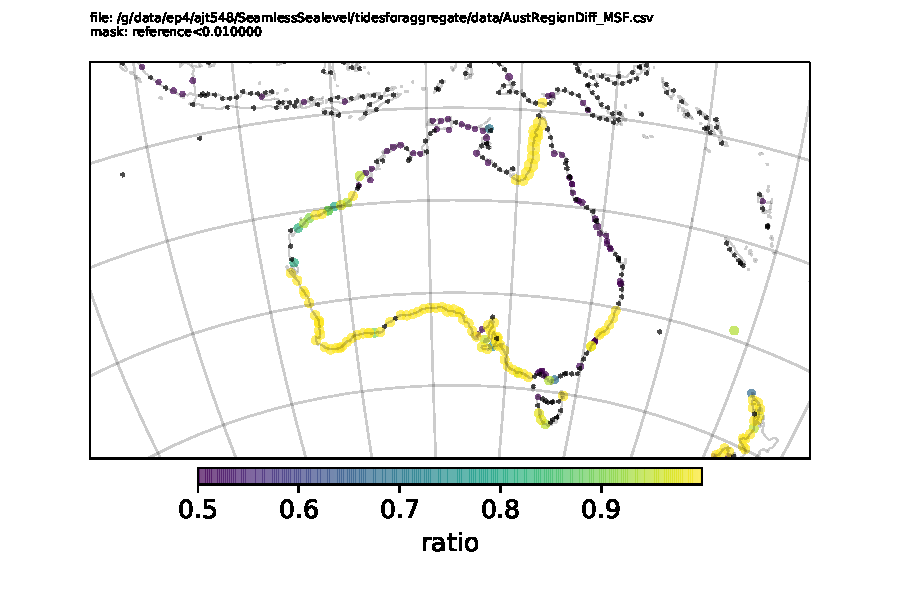
\includegraphics[width=\textwidth]{figures/maps/AustRegionDiff_MSF.pdf}
        \caption{Msf}
    \end{subfigure}
    \begin{subfigure}[b]{\figwidthHalf}
        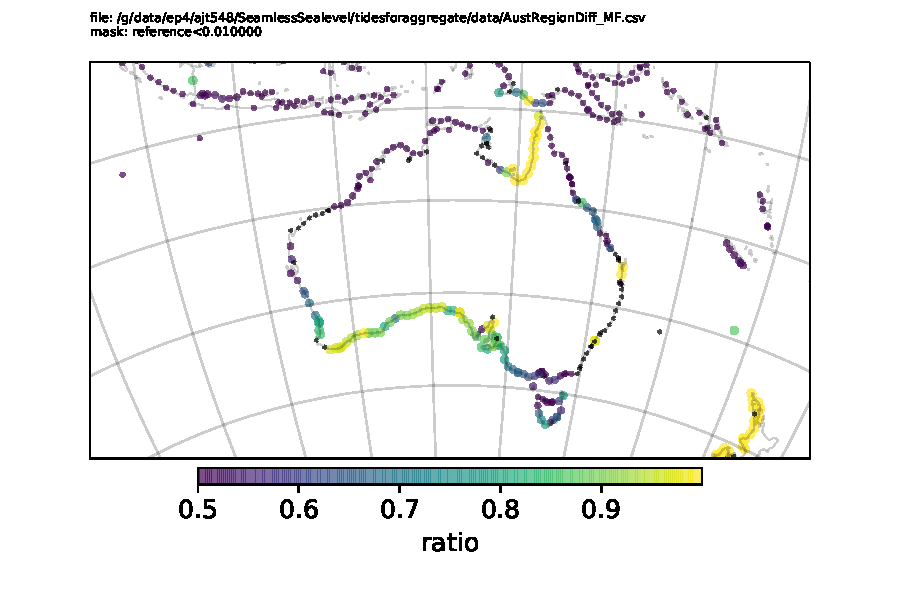
\includegraphics[width=\textwidth]{figures/maps/AustRegionDiff_MF.pdf}
        \caption{Mf}
    \end{subfigure}
    \begin{subfigure}[b]{\figwidthHalf}
        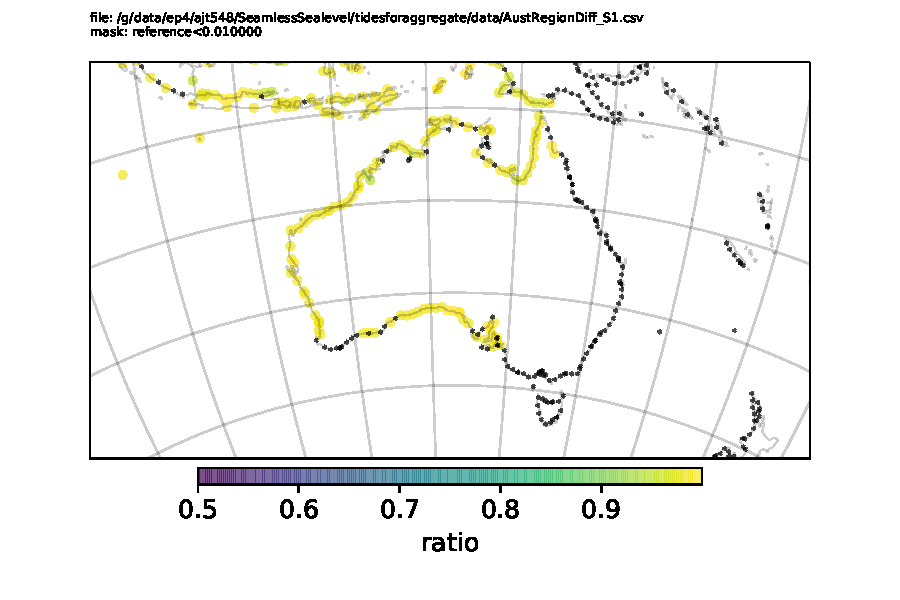
\includegraphics[width=\textwidth]{figures/maps/AustRegionDiff_S1.pdf}
        \caption{S1}
    \end{subfigure}
    \caption{Fractional ratio of tidal amplitude attributed to wind and pressure effects}
    {Data from supplementary material provided by \citet{10.5194/os-2020-107}, based only on amplitude and ignoring magnitudes $<1$cm.  As a starting estimate, the observational-based standard analysis of these constituents could be categorised as primarily non-astronomical.}
    \label{fig:williamsFraction}
\end{figure}

The practical impact of such double-counting is evaluated below using operational sea level data from a system that linearly superposes standard tide parameters with a global ocean circulation forecasts and other inputs at tide gauge locations \citep{Taylor:2017coa,10.1080/1755876x.2019.1685834}.
Figure \ref{fig:aggStatsComet} summarises the skill impact of applying the full standard tide prediction in place of a physical tide estimate that excludes nominally weather dominated constituents. Figure \ref{fig:aggStatsPdf} shows the day-1 error distributions for the same dataset at two example stations.
For these evaluations no bias correction was applied and sample means over approximately 3 years of 1-hourly data are removed.  Whilst the predictive skill characteristics varies between locations, the change from the double-counting scenario (`A' in the figures) to the physical tide scenario (`B') systematically reduces excess variance and improves correlation.

\begin{figure}[!hbt] \centering
    % Taylor
        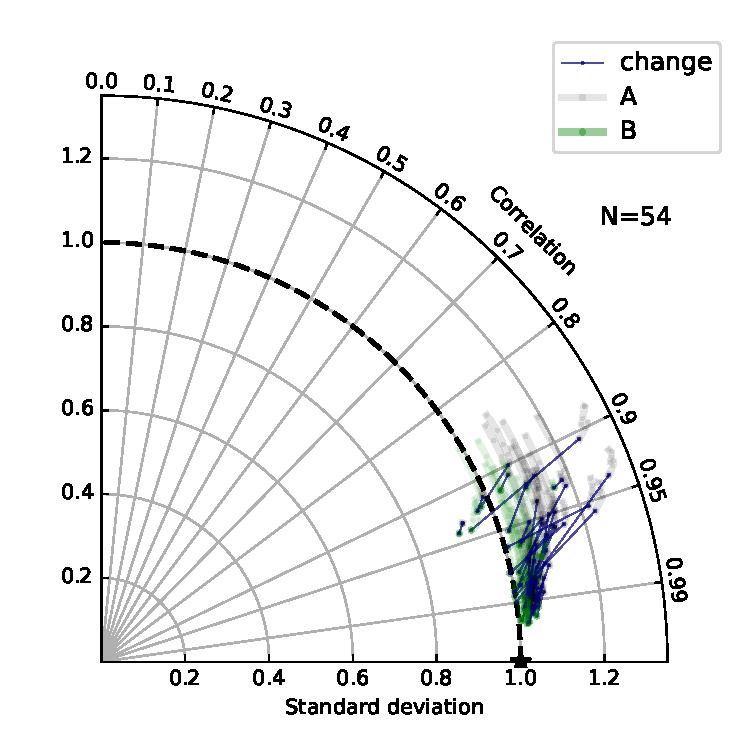
\includegraphics[width=\figwidthBig]{figures/plots/taylorDoubleCount.pdf}
        \caption{Forecast skill decay contrasting two tide prediction variants.}
        {Full forecasts based on linear superposition. Summary of the skill impact due to excluding constituents discussed in the text, across many tide gauge locations. Normalised relative to respective observations \citep{Taylor:2000wp}. Each `comet' traces 7 forecast days.  Change from A to B marked for first day.}   
        \label{fig:aggStatsComet}
\end{figure}   

\begin{figure}[!hbt] \centering
    % D
    \begin{subfigure}[b]{\figwidthHalf}
        \includegraphics[width=\textwidth]{figures/plots/ObsError_\Db.png}
        \caption{\Dname{}}
    \end{subfigure}
    % G
    \begin{subfigure}[b]{\figwidthHalf}
        \includegraphics[width=\textwidth]{figures/plots/ObsError_\Gb.png}
        \caption{\Gname{}}
    \end{subfigure}
    \caption{Day-1 forecast error distribution examples at two sites.}
    {Variants shown are [A] all constituents (official) and [B] exclusion of nominally weather dominated (weather-free).  Operational data for $\sim3$ years. Record means removed.} 
    \label{fig:aggStatsPdf}
\end{figure}   


%------------------------------------------------
\section{Problem 3: constants are not really constant}
\label{Sec:Evolution}
The final problem to motivate the proposed split of tidal data service types is the manner in which tidal parameters vary historically with each annual update.
Australian tidal agencies do not systematically publish the parameters associated with the annual tidal production cycle; expect for the subset of constituent values at select sites that are supplied with the nautical publications \citep{austides}.  The following evaluation is believed to be the first account of the temporal evolution of parameters behind these official predictions.  

Conventional tidal parlance reflects an effective aim for the annual analysis that is to better identify a time-invariant admittance relationship characterised by a set of constants; constants that ideally wouldn't change if only we knew them well enough. \citet{Flinchem:2000kp} characterises this as old clockwork and  line-spectrum framework. 

In contrast, \citet{Colosi:2006va} assert that ``\textit{variability in the values of tidal `constants' should be the rule rather than the exception!}'' 
The expectation of temporal instability for tidal constants has recently been further elaborated by  \citet{10.1029/2018rg000636} and \citet{10.1002/2017jc013165} amongst others.    This reasonable characterisation obviously presents some level of conceptual incompatibility with standard practice.

Inspection of annual changes across the archive of analysis parameters first and foremost highlights the wide range of sources and heterogeneous inputs managed to produce tide tables - as characterised in Figure \ref{fig:tidePractice}.    Whilst the ability to derive value from such a range is a great strength of conventional practice, the resulting predictions  should be accompanied by rankable quality measures as proposed in Section \ref{Sec:proposed}.
The evolution of tidal parameters across the archive is addressed below in two parts relevant to a prospective automated tidal data service:  updates to nominally weather-dominated harmonics and then updates to the separation of MSL from prediction datum.

Of all the sites on the archive, only a subset are based on tide gauges stations that are both in operation and supplying data to the agency for analysis. When new observations are available the annual analysis typically extends the length of record analysed.   The analysis of a continually accumulating record is consistent with the aim of better fitting a set of constants; but is in contrast to studies specifically investigating non-stationary tidal evolution such as \citet{10.1002/2017jc013165}.
As an indication of how actively updated tidal parameters actually are, the full set of well over 600 tidal locations was reduced to around 130 that had any change to the 5 significant figures attributed to M2 amplitude since 2011 - as shown by the reduction in sites between Figures \ref{fig:SaAmp} and \ref{fig:SaPha}.


%--------------------------
\subsection{Harmonics}
To illustrate the evolution of nominally weather-dominated constituents, a set of six tide prediction sites spanning the Australia region are selected and detailed in Table \ref{tab:sites}.  The map in Figure  \ref{fig:SaPha} indicates the geographic location of these sites.
Each of these sites have recent forecasting relevance and real time observations but are in some way challenging from a conventional tidal prediction perspective.   These are mainly \textit{secondary ports} in which the observational record is known to be less than ideal. 
Figure \ref{fig:complexEvolution} shows how these `constants' have evolved over the last decade at the selected sites.   Overall the changes reflect the projection of quasi-periodic signals and growing record length.  

%----------------------------------
% table
%\begin{specialtable}[H]\centering
\begin{tabular}{ r|p{1cm}|p{1.2cm}|c|c|c }
Name 
 & ANTT 
 & BoM 
 & web  
 & port type
 & Obs for 2022
  \\ 
\toprule
Mornington Island 
 & 63540 
 & 529020 
 & Y 
 & Secondary 
 & 30/06/2007 - 31/12/2016
 \\
Christmas Island  
 & 46290 
 & 200970 
 & Y 
 & Secondary 
 & 04/08/2009 - 31/12/2018
 \\
Point Murat       
 & 62430 
 & 005096 
 & Y 
 & Secondary 
 & 13/05/2008 - 31/12/2019
 \\
Geraldton         
 & 62290 
 & 008314 
 & Y
 & Primary   
 & 01/01/1985 - 31/12/2019
 \\
Cape Jervis       
 & 61561 
 & 523757 
 & N 
 & Secondary
 & 29/05/2014 - 31/12/2019
 \\
Lord Howe Island  
 & 57720 
 & 200854  
 & Y 
 & Secondary 
 & 02/08/1994 - 31/12/2019
 
 \\
\end{tabular}
\label{tab:sites}
\end{specialtable}
 
\begin{table}\centering
\begin{tabular}{ r|p{1cm}|p{1.2cm}|c|c|c }
Name 
 & ANTT 
 & BoM 
 & web  
 & port type
 & Obs for 2022
  \\ 
\hline
Mornington Island 
 & 63540 
 & 529020 
 & Y 
 & Secondary 
 & 30/06/2007 - 31/12/2016
 \\
Christmas Island  
 & 46290 
 & 200970 
 & Y 
 & Secondary 
 & 04/08/2009 - 31/12/2018
 \\
Point Murat       
 & 62430 
 & 005096 
 & Y 
 & Secondary 
 & 13/05/2008 - 31/12/2019
 \\
Geraldton         
 & 62290 
 & 008314 
 & Y
 & Primary   
 & 01/01/1985 - 31/12/2019
 \\
Cape Jervis       
 & 61561 
 & 523757 
 & N 
 & Secondary
 & 29/05/2014 - 31/12/2019
 \\
Lord Howe Island  
 & 57720 
 & 200854  
 & Y 
 & Secondary 
 & 02/08/1994 - 31/12/2019
 \\
\end{tabular}
\caption{Selected tidal stations for focus.}
\label{tab:sites}
\end{table}

%----------------------------------

\begin{figure}[!hbt] \centering
    % B
    \begin{subfigure}[b]{\figwidthHalf}
        \includegraphics[width=\textwidth]{figures/plots/complex_\Ba.pdf}\caption{\Bname{}}
    \end{subfigure}
    % C
    \begin{subfigure}[b]{\figwidthHalf}
        \includegraphics[width=\textwidth]{figures/plots/complex_\Ca.pdf}\caption{\Cname{}}
    \end{subfigure} 
    \\
    % D
    \begin{subfigure}[b]{\figwidthHalf}
        \includegraphics[width=\textwidth]{figures/plots/complex_\Da.pdf}\caption{\Dname{}}
    \end{subfigure}
    % E
    \begin{subfigure}[b]{\figwidthHalf}
        \includegraphics[width=\textwidth]{figures/plots/complex_\Ea.pdf}\caption{\Ename{}}
    \end{subfigure}
    \\
    % F
    \begin{subfigure}[b]{\figwidthHalf}
        \includegraphics[width=\textwidth]{figures/plots/complex_\Fa.pdf} \caption{\Fname{}}
    \end{subfigure}
    % G
    \begin{subfigure}[b]{\figwidthHalf}
        \includegraphics[width=\textwidth]{figures/plots/complex_\Ga.pdf} \caption{\Gname{}}
    \end{subfigure}
    \caption{Evolution of select tidal constituents at focus sites.}
    {Histories of annual updates for sites listed in table \ref{tab:sites} displayed as both phasors and smaller timeseries of amplitude and phase.  Annual results are not independent due to accumulating input data. Relatively radical changes reflect the power of quasi-periodic variability at these frequencies as well as the heterogeneous record quality on which analyses are based} 
    \label{fig:complexEvolution}
\end{figure}   

Of the constituents shown, the annual signal \textbf{Sa} is dominant at all of the sites.
Intra-seasonal power and variability is notable at the two sites located in the North West; Port Murat and Christmas Island.   The existence of long period ocean phenomena in this region associated with the MJO atmospheric forcing described by \citet{Maxime:2019jc} should be expected to project onto a conventional tidal analysis.   Internal-tides are of special interest on the North West Shelf \citep{10.3389/fmars.2021.629372} and may also play a role in  modulating surface water level patterns in the manner described by \citet{Colosi:2006va}.

Of the selected sites, Geraldton shows the smoothest and least significant changes.  Given that it is both a \textit{primary port} and based on the longest observational record it may at face value appear to represent the true tidal pattern. But the strong seasonality of the Leeuwin current described by \citet{Ridgway:2004kb} provides an attribution that relies neither on the gravitational tidal forcing nor a barotropic ocean response to weather forcing. % NOTE - anything about the tide gauge boat impact  to add?
This connection is supported by recent attribution studies of sea level along the WA coast, in which historical observations are decomposed using a hybrid tidal and filtering approach to highlight the ``\textit{interesting connection between the probability of extreme sea level events with the large-scale dynamics of an ocean boundary current system}'' \citep{10.1029/2020ef001620}.

Lord Howe Island is located within the eddy the field associated with the East Australian Current and subject to relatively powerful and slow sea level variations.    The parameters fit by the standard tide prediction are quite small and would appear to thus be correctly rejecting the projection of these  non-periodic variations.   However, this site is has been recorded as problematic for the utility of some tide predictions ``\textit{...due to persistent yet sporadically changing ocean levels ...at similar frequencies to the Sa and Ssa constituents [such that] forecasting can then result in errors greater than the actual residual}''\citep{MHL2156}.  The problematic predictions were not based on the analysis of the NTU but rather on a practice of fitting tides to shorter records motivated by the aim of better prediction a useful mean sea level (MSL) for year ahead in the context of inter-annual variability.

%--------------------------
\subsection{Mean sea level}
\label{Sec:MSL}
What mean sea level (MSL) represents for operational purposes and across applications has been singled out as a source of inter-agency inconsistency \citep{MHL2156}.
For studies of sea level average return periods, \citet{Haigh:2013bn} considers MSL to be a time varying background sea level signal.
In contrast, for spatial and survey applications MSL is an important geodetic reference treated as a static value. Furthermore the decomposition of a static MSL to quantify the mean dynamic topography component has a special relevance for datum unification \citep{Filmer:2018cu}.
Applications of tidal predictions that project to periods well beyond the current year such as that described by \citet{10.1007/s11069-021-04600-4} require the ability to separately account for any MSL component.
The official Australian nautical predictions are accompanied by an explanation that highlights to overlap between the concept of MSL and long period tides:
``\textit{Wherever possible, predictions are based on continuous observation of the tide over a period of at least one year, in such cases the average changes in mean sea level due to changes in meteorological conditions for the year in question are calculated and included in the predictions.  These changes do not, however, repeat themselves exactly from year to year; it has been advisable, therefore, to observe and analysis changes in mean sea level for a period of not less than three years.   In case of modern analyses, this practice has been increasingly adopted}'' \citep{austides}

The elevation of MSL relative to \textit{prediction datum} (PD)is updated annually for Australian predictions for multiple reasons.   One is to account for global sea level trends across the prediction sites inclusive of locations for which no recent observations are available.   Other reasons include the redefinition or relocation of PD at a port.  Figure \ref{fig:z0Evolution} summarises the actual historical 
changes in this offset across all Australian primary and secondary ports relative to the arbitrary reference year of 2011.   It is evident that older predictions and lower quality secondary ports are most susceptible to larger step changes.

\begin{figure}[!hbt] \centering
    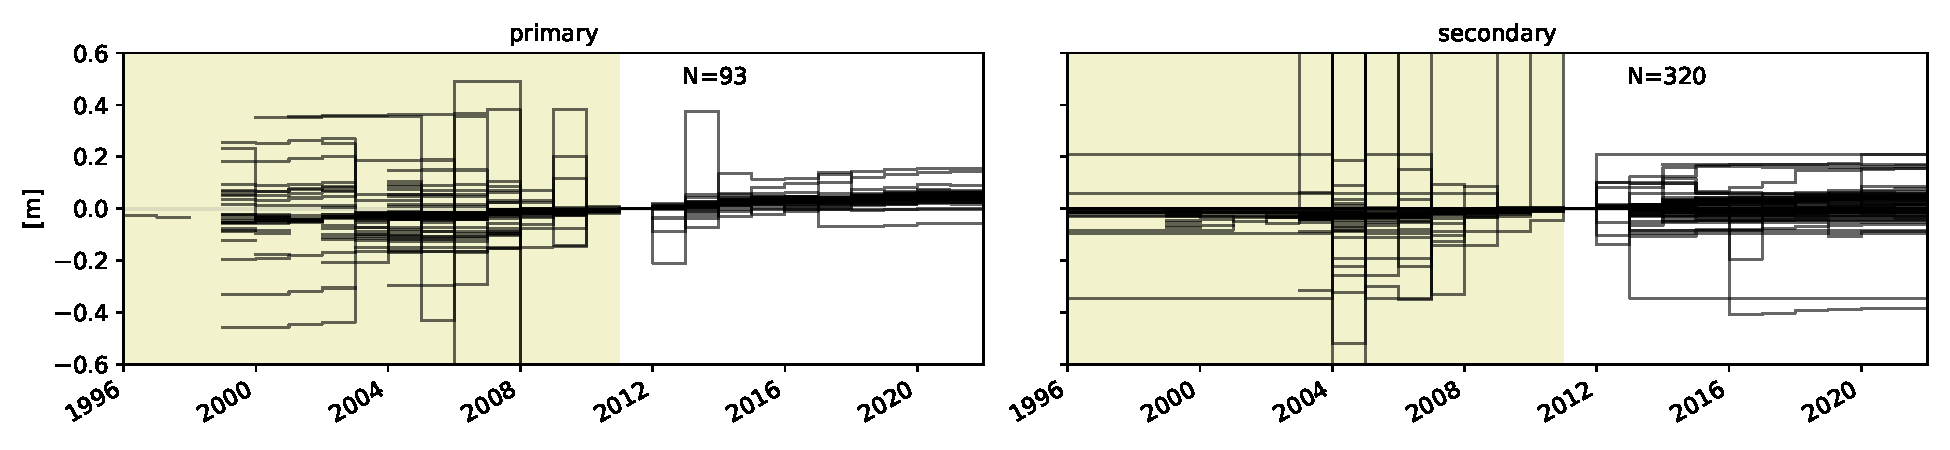
\includegraphics[width=\figwidthFull]{figures/plots/Z0_evolution.pdf}
        \caption{Evolution of zero frequency levels used for annual tide predictions at Australian primary and secondary ports. }
        {Each line represents a single station and traces the change in zero frequency level values relative to arbitrary zero year of 2011. More discontinuous updates are apparent for predictions in the early period and for secondary ports; reflecting the heterogeneity of sources and potential for offset discontinuities with on-demand data delivery.  The vertical scale of the second panel is intentionally clipped to match that of the primary ports.}
    \label{fig:z0Evolution}
\end{figure}   

\subsection{Relevance of annual updates for a data service}
The annual update to official parameters is undertaken with the specific goal of improving stand-alone water level predictions for the year ahead.  It should come as no surprise that this practice may introduce discontinuities when looking back over historical predictions.
But looking back at official data is exactly what some users of an automated data service may require and it is important that there is no confusion about what data is being supplied.
Compare this to an application where the aim is simply to estimate the tidal water level variability component  for a historical period regardless of what was official or available at the time.
Figure \ref{fig:tideHistoryTs} illustrates the difference for the case of  \Dname{}.  The evolving long period characteristics of the official annual updates can be compared to panel [c] in Figure \ref{fig:complexEvolution} recalling that these operational values represent a growing input record and an independent observations such in the studies of \citet{10.1002/2017jc013165}. 

\begin{figure}[!hbt] \centering
    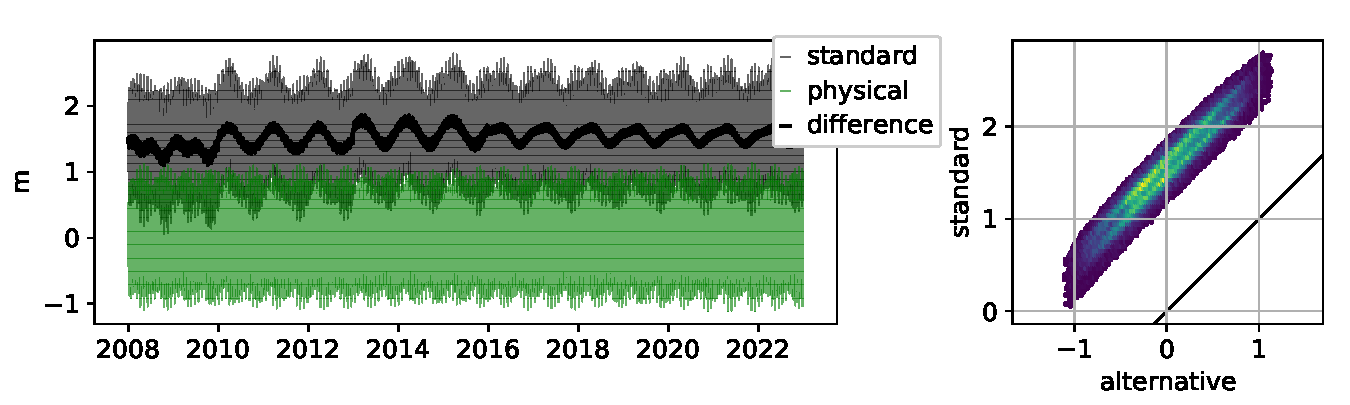
\includegraphics[width=\figwidthFull]{figures/plots/piecewiseTide_62430.pdf}
        \caption{Contrast between concatenated standard predictions and an alternative physical hindcast.}
        {Illustrated by hourly tide prediction variants for \Dname{}. The left panel overlays standard and physical variants across the period 2008 to 2023, and shows the houlr differnce timeseries in green. The hindcast shown is based on the approximate ``weather-free'' tidal parameters.  In addition to the constant offset, intentional discontinuities are apparent in official predictions associated with annual updates and growing input record length.  The right planel compares the same two multi-year timeseries as a scatter of contemperanous hourly samples; both axes show prediciton heights in metres.}
    \label{fig:tideHistoryTs}
\end{figure}   

%------------------------------------------------
\section{Proposed split of routine tidal content}
\label{Sec:proposed}
The above sections have characterised the place of conventional tidal practice alongside operational oceanography within a forecasting agency and described three problems that could impact the value of a singular implementation of a machine-readable tidal data service.   From this starting point, the current section proposes a direction by which the conventional service may incrementally adapt to modern requirements.  This proposal is written from the premise that the very notion that anything other than a singular tide prediction is required represents a significant conceptual shift for conventional practice.
Adding any complexity to operational systems is generally undesirable and a good data service just ``does what it says on the box''.  But considering the diverse uses for synthesised tidal signals and the problems outlined above, the following aims for a data service are put forward: 
\begin{itemize}
    \item deliver tide data valid for arbitrary times
    \item isolate users from details of backend software 
    \item distinguish a physical tide estimate from standard predictions
    \item allow for differentiation between forecasts, hindcasts and analyses
    \item visibility of reference datum and MSL change components
    \item provide rankable quality measures
\end{itemize}

With these motivations in mind, a minimal set of tidal data categories are proposed and listed in table \ref{tab:typesSummary}.   Emphasis is placed on conveying the need for \textit{any} signal split rather than exact wording and finer details.  Importantly, such a change could be made as an incremental shift without significant technological change; but would open the path to ongoing improvements in the respective categories. 
Each is discussed further in the subsequent sections.

%\begin{specialtable}[H]\centering
\begin{table}[H]\centering
    \begin{tabular}{ |c|c|c|c|c| }
    \hline
    name    & 
        default reference  & 
        issue date         & 
        valid time limits  \\
    \hline
    standard tide prediction [\ref{Sec:flavour1}] & 
        chart datum & annual & 
        concatenated bounds\\
    \hline
    physical tide prediction [\ref{Sec:flavour2}]& 
        MSL       & 
        arbitrary & 
        no limit \\
    \hline
    physical tide analyses [\ref{Sec:flavour3}]& 
        MSL       & 
        arbitrary & 
        within observation range \\
    \hline
    \end{tabular}
    \caption{Summary of proposed timeseries data categories; metadata are addressed in \ref{sec:spatial} and \ref{sec:quality} }
    \label{tab:typesSummary}
%\end{specialtable}
\end{table}
These proposed incremental changes for the conventional service should not be confused with the vital role of global repositories of sea level observations \footnote{such as \url{www.gloss-sealevel.org}, \url{uhslc.soest.hawaii.edu} and \url{www.gesla.org}}.    The starting premise of this discussion is the ongoing and embedded role of the national agency for conventional tidal services.    
Similarly, global simulation repositories like that described by \citet{10.3389/fmars.2020.00263}
serve an important but different role.

%------------------------
\subsection{Standard reference predictions}
\label{Sec:flavour1}
Standard tide predictions have an official legal status both directly for navigation purposes and indirectly for some other applications.   
For instance the Australian Navigation Act \citep{AusNavAct2012} details a requirement for vessels to carry nautical publications, and specifically tide tables, from the official charting authority.  Charted depths are defined relative to a datum generally aligned with the Lowest Astronomical Tide value derived from synthesised official tidal timeseries over a fixed period \citep{PCTMSL-sp9}.

% reviewer input on legal
Official tide predictions are not \textit{directly} connected to cadastral definitions in Australia, but may often play an indirect role in the determination of boundary references such as `mean high water mark' \citep{NSW_spatial2012} or the `intertidal zone' \citep{BlueMud_2017}.

%Official predictions are forecasts that aim to represent the total still-water level under average conditions. ``\textit{As predictions are given for average meteorological conditions it follows that when conditions are not average the actual tides may differ from those predicted.}''\citep{austides}
Official predictions traditionally cover a fixed validity period of one year and are issued on an annual update cycle well in advance; for instance the 2022 predictions may be issued in late 2020.  An on-demand data service should allow users to access these predictions at arbitrary timestamps within the validity period, and conventional needs such as high and low waters just represent a special timeseries subset.
As described in section \ref{Sec:Evolution}, discontinuities should be expected between these annual official predictions. 
Providing access to \textit{historical} predictions therefore requires a data-service to appropriately handle the forecast validity dates.  Whilst this requirement precludes the use of a single set of tidal parameters to synthesise a hindcast on-demand, it does not rule out on-demand synthesis in general.
Tidal planes associated with official predictions, such as LAT and HAT, should similarly be accessible according to validity period.

%------------------------
\subsection{Physical or `weather-free' tidal timeseries}   
\label{Sec:flavour2}
As described in the preceding sections, there are valid use-cases for tide predictions that do not align with the aims of standard products;  both with respect to the ``official'' status of the annual promulgation and as well as the component of observable sea level that is being targeted.  It is asserted that many such cases require the best available estimate of the tidally-driven component of total sea level.  
Following the evaluations in sections \ref{Sec:OfficialGlobal}and\ref{Sec:DoubleCount} it is asserted that a reasonable approximation to such a physical prediction could be made with existing methods by bluntly removing tidal constituents that are determined to be weather-dominated; specifically all of the long period tides and S1.   Such an approximation is proposed as an adequate and immediately available tidal variant that could be refined in isolation to official prediction constraints. Furthermore, the role of charting PD is unlikely to be relevant to these applications and should be default be excluded.
There is no reason to restrict the refinement of analysis parameters to an annual update cycle.
Such a prediction is simply what physical oceanography has largely thought of as `tides' for decades \citep{Munk:1966ts} despite the fact that response method techniques ``\textit{...have never been adopted for ordinary tide-table production [and] remain essentially a research tool for specialists}''\citep[p.198]{Cartwright:2000tt}.
Combination with dynamic model forecasts requires such a prediction \citep{Taylor:2017coa}, as does any data-driven methodology that involves the filtering of real-time tide gauge observations in order to assimilate non-tidal residuals \citep{10.3389/fmars.2019.00437}. Furthermore, residuals derived using such a weather-free tide prediction prima facie share the representational targets of sea level anomaly (SLA) data derived from satellite altimetry as discussed section \ref{Sec:OfficialGlobal}.
      
%------------------------
\subsection{Behind-real-time quality tidal timeseries}  
\label{Sec:flavour3} 
Whereas a tidal hindcast can be synthesised for a past period with no methodological difference to a forecast, there is a reason to conceptually separate this from an analysis timeseries. The dual meaning of 'analysis' for both the tidal process and the timeseries here is unfortunate but unavoidable and hopefully clarified by context. 
The distinction being analogous to that between a weather model forecast and analysis, or the IGDR and GDRs of satellite data \citep{Picot:2003tp}.    As a starting approximation this data category would be served by conventional methods but only valid for the time span of the input observations. 
Distinguishing this data category would serve the role of a de-tiding filter for historical observations, as an evaluation target for behind-real-time regional tide modelling like that of \citet{10.5194/os-2020-107} and potentially as an input to geophysical re-analysis (eg \citep{10.1029/2017jc013685}).    
In contrast to the use of a constant set of tidal parameters to synthesise a prediction or hindcast, keeping this category separate would allow for the application of non-stationary methods to account for modulation and transient phenomena that can still be usefully attributed to tides as per the discussion of wavelet and other techniques by \citet{Flinchem:2000kp}. 

%------------------------
\subsection{Spatial metadata and levels}
\label{sec:spatial}
Metadata regarding the location, identity and especially relative elevation of tidal timeseries is fundamental to any data service.
Vertical datum transformation and unification is an active area of development is Australia and described in \citet{Keysers:we} and \citet{Filmer:2018cu} amongst others.   Spatial reference developments such as the Australian Vertical Working Surface are notably also connected to tidal observations \citep{AVWS2021}).   The details are beyond the scope of the present discussion, but the relationship between prediction datum and the ellipsoidal references employed in modern positioning\footnote{\url{ https://www.icsm.gov.au/what-we-do/aushydroid}} is highlighted as carrying special relevance.

%------------------------
\subsection{Rankable quality measures}
\label{sec:quality}
Whilst high quality, continuous long records of sea level observation represent an ideal for conventional tidal methods, in practice this is only available for a relatively small network of tide gauges.   
The schematic in Figure \ref{fig:tidePractice} conveys the attractive ability of conventional tidal practice to produce uniform outputs from a very heterogeneous set of inputs.
Uniformity of format is not the same as uniformity of quality, but without appropriate supporting information users of tidal data would be left to treat all predictions as equal.  

Australian systems currently have effectively only two quality categories: `primary' and `secondary' \citep{austides} that are sometimes also designated `standard' and `subordinate'  \citep{PCTMSL-sp9}.   
It is also common to see unofficial tide predictions clearly marked as ``not for navigation'' to indicate a status other than official.
This binary classification is not sufficient for many applications and it is asserted that the major deficiency is the lack of ability to rank by quality.   There are several dimensions by which synthesized tidal timeseries could be assigned rankable quality measures.    
The analysed observational record length is at least one practical candidate and specifically highlighted by \citet{MHL2156}. But the bespoke analysis process, for instance involving inference or moved stations \citep{godin:1972}, can render record length more ambiguous than at first may be apparent.    
Related to record length is the candidate measure of extrapolation time, to quantify the time period prior-to or after the analysed observational record.     
A quality measure that reflects skill relative to an independent period of water level observations could also provide useful guidance to users of the data.    In contrast, any measure derived directly from the tidal analysis itself (inversion) would require care to avoid over-fitting and the type of circular reference described by  \citet{Thompson2019}. 

The absence of rankable quality measures left \citet{10.5194/os-2020-107} to rely on a needlessly empirical blacklisting procedure to reject tidal analysis sites from a simulation evaluation on the basis of being of grossly poor quality. Such information should readily accompany machine-readable tidal data.

%------------------------------------------------
\section{Concluding discussion}
\label{Sec:Discussion}
This article has put the case that an appropriate clarification of tidal data types and aims will enable a conventional tide prediction service to better compliment a range of modern applications; and that such a change could be relatively incremental and feasible with existing technology. 
There is of course a very long history of proposals for refinements or up-ending of tide prediction techniques \citep{Cartwright:2000tt,Jay:2003bj}, but in contrast the present argument is for an incremental shift in the thinking behind an established and valuable \textit{service}.
The magnitude of the signals and discontinuities are overall rather small at only $\sim10-20cm$.   But scales like this are worthy of attention when considering the operational role for forewarning of nuisance flooding \citep{Devlin:2017hu,10.1071/es19024} and potentially in complimenting future remote observation platforms \footnote{\url{auswot.org}} and coastal forecasting more generally \citep{10.3389/fmars.2019.00437}.

This discussion has intentionally not promoted the promulgation of tidal analysis parameters and has instead focused on the value of timeseries services.   
Whilst transparency of prediction methods and parameters is of itself desirable, the publication of tidal constants is less likely to directly deliver the value required by downstream applications.    Most simply because the interpretation and application of tidal constants requires consistency between the analysis and synthesis software. 

A technically trivial but serious case is the known inconsistent designation of \textbf{Sa} to Doodson numbers \texttt{[0 0 1 0 0 0]} and \texttt{[0 0 1 0 0 ‐1]} between tools \citep{PCTMSL-sp9}.  

More generally, supplying tidal constants as a service raises deeper uncertainties regarding the varying manner in which non-stationary signals are either projected onto named constituent groups or even incorporated into predictions (eg \citep{Matte:2012df}). 
Providing timeseries would directly serve many direct downstream applications as well as allowing specialist users to `back out' parameters in their own analysis framework as required and in isolation from the details of tools in use by the supplier.



Moving towards a differentiated micro-service \citep{BCG2020} approach to supplying conventional tidal data would be a step in the right direction for the National agency.
